% !TeX root = ../main-english.tex
% !TeX spellcheck = en-US
% !TeX encoding = utf8
% -*- coding:utf-8 mod:LaTeX -*-

%This smart spell only works if no changes have been made to the chapter
%using the options proposed in preambel/chapterheads.tex.
\setchapterpreamble[u]{%
	\dictum[John Claerbout, paraphrased by Buckheit \& Donoho]{An article about computational science in a scientific publication is not the scholarship itself, it is merely advertising of the scholarship. The actual scholarship is the complete software
	development environment and the complete set of instructions which generated the figures.}
}


\chapter{Ensuring computational reproducibility across computational environments}
\label{chap:k3}


Partially fueled by funding mandates (CITATION needed) and research curricula founded within the Open Science Movement (CITATION NEEDED), practices of publishing reproducibly and reproducing published results are becoming more frequent.
Grass-roots movements such as Reprohack (\href{https://www.reprohack.org/}{www.reprohack.org}) or the ``Ten Years Reproducibility Challenge'' (\href{https://rescience.github.io/ten-years/}{rescience.github.io/ten-years}) train researchers to check published studies for reproducibility.
Widespread sharing of code and data allows researchers to verify, reuse, and improve upon past work of others (CITATION NEEDED).
Consequently, though, attempts to reproduce previous studies often happen in different computational environments than those that originally created the results in question.
Ensuring computational reproducibility across computational environments is, however, a difficult technical challenge.
This following chapter outlines first its challenges, particularly in the field of neuroimaging, then its opportunities, and lastly an implementation to ensure computational reproducibility across computational environments.
Parts of this chapter were published as \citet{wagner2022fairly}: ``FAIRly big: A framework for computationally reproducible processing of large-scale data'' and are appropriately marked as such.


\subsection{Terminology}

Over the past decade, so-called \textit{reproducibility crises} in numerous fields have increased the interest of the scientific community and funders in reproducibility (CITATION NEEDED) \citep{wagner202310}.
However, proposals to increase reproducibility, transparency, and robustness of science were made independently in various disciplines long before the current trend, in some cases dating back several centuries (maybe Robert Boyle, chemistry CITATION NEEDED).
Even the field of \textit{computational reproducibility} -- despite increased usage of the term in scientific literature only from 2015 onward (see \cref{fig:ngram}) -- originated already more than 30 years ago in the field of seismology \citep{claerbout1992electronic} \citep{buckheit1995wavelab}.
Consequently, the terminology around reproducibility has varied considerably over the years and across domains, and there is no universally agreed upon standardization of terminology in place yet \citep{barba2018terminologies}.
To disambiguate between several conflicting definitions of terms around reproducibility that are in active use, we shall define the terms used in this thesis as follows: \\
Following the definition of \citet{peng2006}, \textit{reproducibility} refers to the practice of verifying a published result with the same methods and materials used by the original authors. \\
\textit{Replicability}, on the other hand, refers to strengthening scientific evidence in favor of a result when ``multiple investigators [find similar results] using independent data, analytical methods, laboratories, and instruments''  \citep{peng2006}. \\
\textit{Computational reproducibility}, finally, matches to the definition put forward in the 2019 report on ``Reproducibility and Replicability in Science'' by the National Academies of Science, Engineering and Medicine \citep{engineering2019reproducibility}: ``We define reproducibility to mean computational reproducibility – obtaining consistent computational results using the same input data, computational steps, methods, code, and conditions of analysis''.


\begin{figure}
	\centering
	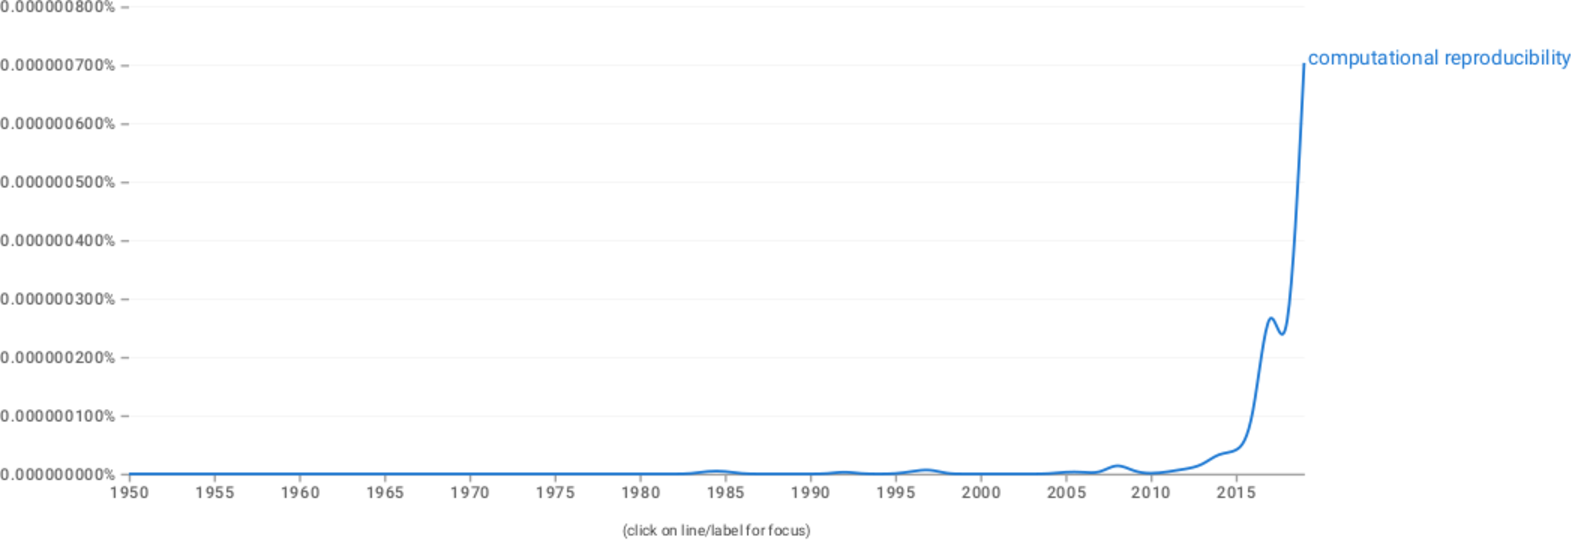
\includegraphics[width=\textwidth]{google_ngram_reproducibility_2023-05-08.pdf}
	\caption{Popularity of computational reproducibility: A chart of the frequencies of the n-gram ``computational reproducibility" (using yearly count, normalized be the numbers of books published in each year) in literature included in the English(2019) corpus of Google books. This graph has been created using the Google Ngram Viewer (\href{https://books.google.com/ngrams/info}{books.google.com/ngrams}) \citep{michel2011quantitative}}
	\label{fig:ngram}
\end{figure}



\pagebreak

\section{FAIRly big: A framework for computationally reproducible processing of large-scale data}
\pagebreak